In the previous chapter, we discussed the problem of anomaly detection in time series.
This chapter is devoted to providing some concepts and methodologies which are addressed in our work. 
We will cover different statistical time series models in general terms and introduce our notation. 
Subsequently, we will address learning and inference methods in such models.
Afterward, we will cover the deep learning sequence models.

The entropy maximizing model for the set of observation $x_{1:T}=\{x_1, x_2, ..., x_{\mathcal{T}}\}$ is to assume the instances are independent and identically distributed (i.i.d.) random variables (RV)\cite{hoadley1971asymptotic}. 
However, in the context of the time series, it is natural to consider models consistent with the causal nature of time \cite{barber2010graphical}. 
So, we can get the following causal form of joint distribution $p(x_{1:\mathcal{T}})$ by applying Bayes' rule recursively:

\begin{eqnarray}
    p\left(x_{1 : \mathcal{T}}\right) & = & p\left(x_{\mathcal{T}} \mid x_{1 : \mathcal{T}-1}\right) p\left(x_{1 : \mathcal{T}-1}\right) \\
    & = & \prod_{t=1}^{\mathcal{T}} p\left(x_{t} \mid x_{1 : t-1}\right)
\end{eqnarray}

This representation of time series has natural causal interpretation in which observations depend on all the past information. 
This phenomenon corresponds to the cascade graph, shown in Figure~\ref{Markov:cascade}, which is the most general form of belief network. 
Obviously, it is an intractable and expensive problem for a large scale model.

\begin{figure}
\centering
    \subfigure[Cascade graph for time-series]{
        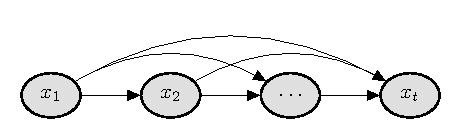
\includegraphics[width=0.9\textwidth]{cascade.pdf}
        \label{Markov:cascade}
    }%
    
    \subfigure[Second-order Markov model]{
        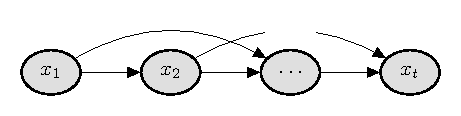
\includegraphics[width=0.9\textwidth]{second_order.pdf}
        \label{Markov:second_order}
    }%
    
    \subfigure[First-order Markov model]{
        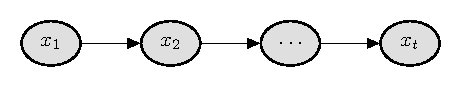
\includegraphics[width=0.9\textwidth]{first_order.pdf}
        %\caption{First-order Markov model}
        \label{Markov:first_order}
    }
    \caption{Graphical models for different time-series models}
    \label{Markov}
\end{figure}

The fundamental solution to this problem is the assumption of conditional independence. 
Intuitively, it corresponds to the removal of the edges in the cascade graph. 
One of the most well-known models for conditional independence assumption on time-series model is the Markov model. 
In which, $L$th-order Markov model assumes that given observation only depends on previous $L$ observations. 
Mathematically, assumption of the $L$th-order Markov model is as the following:

\begin{eqnarray}
    p\left(x_{t} \mid x_{1 : t-1}\right) & = & p\left(x_{t} \mid x_{t-L : t-1}\right)
\end{eqnarray}

Although $L$th-order Markov model is a simplified representation of the cascade graph, it still has relatively high complexity. 
On the other hand, the most straightforward representation of the Markov model is the $1$st-order Markov model, which assumes each observation in the sequence only depend on previous observation. 
It seems easy; however, it has a traceable posterior distribution, and therefore, it is an influential model which allows stronger modeling.
Mathematical interpretation of the first-order Markov model is as follows:

\begin{eqnarray}
    p\left(x_{t} \mid x_{1 : t-1}\right) & = & p\left(x_{t} \mid x_{t-1}\right)
\end{eqnarray}

Graphical models for cascaded graph, second($L$th)-order Markov model and first-order Markov model are shown in Figure~\ref{Markov:second_order} and Figure~\ref{Markov:first_order}, respectively. 
The complexity increases with the order of the network.

\section{Hidden Markov Model}
Up to the present, we examined the models which are directly built on observations.
However, such models are suffering from low representation power on data.
The reason for this is that observations are not always accurate and can deceive the model. 
Therefore, in the literature, a more general framework of time series models exists which uses latent, unobservable variable $s_t$, which generates observations.

From now on, instead of building models where observations depend on previous observations, we build models in which the observations depend on the hidden variable.
One of the most well-known models with this structure is the `state-space models' (SSM). 
In this model, each observation is assumed to be generated from a latent (or hidden) variable.
Therefore, Markov structure is formed on latent variables, $s_{1:\mathcal{T}}$, not on the observations, $x_{1:\mathcal{T}}$.
The observed variables are dependent on the hidden variables through an emission, $p\left(y_t \mid x_t\right)$\cite{barber2012bayesian}. 
Hidden Markov Model is the particular case of SSM in which hidden variables are only dependent on the previous hidden variable \cite{rabiner1989tutorial}.
Hence, state-transition dynamics are shown as $p\left(s_{t} \mid s_{t-1}\right)$.
In other words, Hidden Markov models are first order state-space models. Graphical model for HMMs is given in Figure~\ref{fig:hmm}. The joint probability distribution for this model is given below.
Initial state $s_1$ can be considered as dependent on initial hidden state $s_0$ and $p\left(s_1\right) = p\left(s_1 \mid s_0\right)$ so that one could get a simpler expression for joint probability.

\begin{eqnarray}
    p\left(s_{1 : \mathcal{T}}, x_{1 : \mathcal{T}}\right) & = & \left[\prod_{t=1}^{\mathcal{T}} p\left(x_{t} \mid s_{t}\right)\right]\left[\prod_{t=2}^{\mathcal{T}} p\left(s_{t} \mid s_{t-1}\right)\right]p\left(s_{1}\right) \\
    & = & \prod_{t=1}^{\mathcal{T}} p\left(x_{t} \mid s_{t}\right)p\left(s_{t} \mid s_{t-1}\right)\label{eq:hmm}
\end{eqnarray}

\begin{figure}
    \centering
    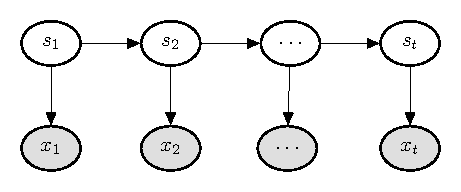
\includegraphics[width=0.9\textwidth]{figures/hmm.pdf}
    \caption{Graphical model for hidden Markov models or first-order state-space models}
    \label{fig:hmm}
\end{figure}

There are different naming for hidden Markov models because both discrete and continuous models share the same graphical model structure. 
For the convention, we use the term `state-space models'(SSM) as a generic name for latent state Markov models, `hidden Markov Model'(HMM) for the discrete latent state Markov models and `linear dynamical systems'(LDS) for continuous latent state Markov models.

The hidden variables in HMM are always discrete, while observations could be both discrete or continuous.
Therefore for a HMM, in the case of $S$ different states, the state transition distribution $p(s_{t}\mid s_{t-1})$ can be defined by an $S \times S$ transition matrix {\boldmath$\Psi$} and, $\Psi_{\hat{s}, \hat{s}^{\prime}}=p\left(s_{t}=\hat{s} \mid s_{t-1}=\hat{s}^{\prime}\right)$ denotes the probability of going from state $\hat{s}^{\prime}$ to state $\hat{s}$ at the time $t$. 
It is important to note that the transition matrix {\boldmath$\Psi$} is build from non-negative entries $\Psi_{\hat{s}, \hat{s}^{\prime}}$, and sum of entries in columns of transaction matrix is equal to 1, $\sum_{\hat{s}} \Psi_{\hat{s}, \hat{s}^{\prime}} = 1$
Similarly, in the case of $X$ discrete observations, emission distribution $p(x_t | s_t)$ can be defined  by $ X \times S$ emission matrix {\boldmath$\Omega$} and $\Omega_{\hat{x}, \hat{s}} = p\left(x_t = \hat{x} \mid s_t = \hat{s} \right)$. If the output is continuous then $s_t$ selects one of the potential $S$ output distributions $p(x_t \mid s_t)$.

\section{Inference in Hidden Markov Model}
\label{section:Inference-in-HMM}

Hidden Markov models have widespread applications with different purposes in many different domains, such as speech recognition, bioinformatics, and time series forecasting. Therefore, different outputs and statistics from the model may be requested.
One may try to infer the current latent state $s_t$ from the observations $x_{1:t}$. Mathematically, it can be shown as $p\left(s_t\mid x_{1:t}\right)$. 
This approach is named as {\it filtering} in the literature. 
On the other hand one can try to infer the past $p\left(s_{t-L}\mid x_{1:t}\right)$ or try to infer the future $p\left(s_{t+L}\mid x_{1:t}\right)$ with positive $L$, 
which are known as {\it smoothing} and {\it prediction} respectively. 
Finally one can try to identify the most likely hidden path $\arg\max_{s_{1 : \mathcal{T}}} p\left(s_{1 : \mathcal{T}} \mid x_{1 : \mathcal{T}}\right)$ which is known as {\it Viterbi path}. and can be calculated with {\it Viterbi algorithm}.
In the following parts, we will discover these methods.

\subsection{Filtering}
Filtering is the estimation of the current hidden state by using all observations so far, $p\left(s_t \mid x_{1:t}\right)$. 
To compute that, one can first find joint marginal $p\left(s_t,x_{1:t}\right)$ which is proportional to conditional marginal $p\left(s_t\mid x_{1:t}\right)$ and conditional marginal can be reached by the normalization.

\begin{eqnarray} 
p\left(s_{t}, x_{1 : t}\right) & = & \sum_{s_{t-1}} p\left(s_{t}, s_{t-1}, x_{1 : t-1}, x_{t}\right) \\ 
& = & \sum_{s_{t-1}} p\left(x_{t} \mid x_{1 : t-1}, s_{t}, s_{t-1}\right) p\left(s_{t}\mid x_{1 : t-1}, s_{t-1}\right) p\left(x_{1 : t-1}, s_{t-1}\right)\\ 
& = & \sum_{s_{t-1}} p\left(x_{t} \mid s_{t}\right) p\left(s_{t} \mid s_{t-1}\right) p\left(s_{t-1}, x_{1 : t-1}\right) \label{eq:filtering}
\end{eqnarray}

If we define $\alpha \left(s_t\right) = p\left(s_{t}, x_{1 : t}\right)$ and put that in the equation \ref{eq:filtering} we could get {\it $\alpha$-recursion} or {\it forward recursion};

\begin{eqnarray}
    \alpha\left(s_{t}\right) & = & \underbrace{p\left(x_{t} \mid s_{t}\right)}_{\text { corrector }} \underbrace{\sum_{s_{t-1}} p\left(s_{t} \mid s_{t-1}\right) \alpha\left(s_{t-1}\right)}_{\text { predictor }} \label{eq:filtering2}
\end{eqnarray}

where $\alpha \left(s_1\right) = p\left(x_{1}, s_{1}\right) = p\left(x_{1} \mid s_{1}\right)p\left(s_{1}\right)$. This recursive formula shows that filtered distribution $\alpha(.)$ is propagated through forward in each step and it acts like a `prior' distribution for the following time step. In other words, at each time step the previous posterior becomes the new prior \cite{barber2012bayesian}.

\subsection{Smoothing}

Smoothing is basically the estimation of the past from the given data.
Mathematically it can express as $p(s_t\mid x_{1:\mathcal{T}})$ where the $\mathcal{T}$ is usually the length of the sequence.
Similar to what have we done in the previous section, we calculate the joint marginal $p(s_t,x_{1:\mathcal{T}})$ instead of conditional marginal.
There are two main approaches to calculate smoothing: {\it Parallel Smoother} and {\it Sequential Smoother}.

\subsubsection{Parallel Smoother}

In this approach, the posterior distribution is rewritten in the form with contributions from the past and the future, taking advantage of {\it d-separation} in the equation \ref{eq:d-seperation}. 
It is the best-known smoothing method in the literature \cite{rabiner1989tutorial}.
Algebraically it can be shown as follows.

\begin{eqnarray}
    p\left(s_{t}, x_{1 : \mathcal{T}}\right) & = & p\left(s_{t}, x_{1 : t}, x_{t+1 : \mathcal{T}}\right) \\
    & = & p\left(s_{t}, x_{1 : t}\right)p \left(x_{t+1 : \mathcal{T}} \mid s_{t}, x_{1 : t}\right) \\
    & = & \underbrace{p\left(s_{t}, x_{1 : t}\right)}_{\text { past }} p \underbrace{\left(x_{t+1 : \mathcal{T}} \mid s_{t}\right)}_{\text { future }} \label{eq:d-seperation}\\
    & = & \alpha\left(s_t\right)\beta\left(s_t\right)
\end{eqnarray}

where $\beta(s_t)$ is called as {\it $\beta$-recursion} or {\it backward recursion}. 
Since $\alpha(.)$ and $\beta(.)$ recursions are independent of each other, and they may be run in parallel. 
So, we have to derive the $\beta$-recursion as in the equation \ref{eq:backward}. It is as follows:

\begin{eqnarray} 
p\left(x_{t+1:\mathcal{T}} \mid s_{t}\right) & = & \sum_{s_{t+1}} p\left(x_{t+1}, x_{t+2:\mathcal{T}}, s_{t+1} \mid s_{t}\right) \\ 
& = & \sum_{s_{t+1}} p\left(x_{t+1} \mid x_{t+2 : \mathcal{T}}, s_{t+1}, s_{t}\right) p\left(x_{t+2:\mathcal{T}}, s_{t+1}\mid s_{t}\right) \\
& = & \sum_{s_{t+1}} p\left(x_{t+1} \mid s_{t+1}\right) p\left(s_{t+1} \mid s_{t}\right) p\left(x_{t+2:\mathcal{T}} \mid s_{t+1} , s_{t}\right) \\
& = & \sum_{s_{t+1}} p\left(x_{t+1} \mid s_{t+1}\right) p\left(s_{t+1} \mid s_{t}\right) p\left(x_{t+2:\mathcal{T}} \mid s_{t+1}\right) \label{eq:backward} \\
\beta(s_t) & = & \sum_{s_{t+1}} p\left(x_{t+1} \mid s_{t+1}\right) p\left(s_{t+1} \mid s_{t}\right) \beta\left(s_{t + 1}\right)
\end{eqnarray}

This $\alpha - \beta$ recursion is known as {\it Forward-Backward} algorithm. Smoothed posterior can be obtained by the normalization of the result of the {\it Forward-Backward} algorithm.

\subsubsection{Sequential Smoother}

In this approach, the recursion is directly formed for smoothed posterior.
In the literature, it is known as {\it correction smoother}. This method also uses the power of the {\it d-separation} in a different manner. 
It makes future observations unnecessary by the conditioning on the latent present state \cite{rauch1965maximum}.

\begin{eqnarray}
    p\left(s_{t} \mid x_{1 : \mathcal{T}}\right) & = & \sum_{s_{t+1}} p\left(s_{t}, s_{t+1} \mid x_{1 : \mathcal{T}}\right) \\
    & = & \sum_{s_{t+1}}p\left(s_{t} \mid s_{t+1} , x_{1 : t}, x_{t+1:\mathcal{T}}\right)p\left(s_{t+1} \mid x_{1:\mathcal{T}}\right) \\
    & = & \sum_{s_{t+1}}p\left(s_{t} \mid s_{t+1} , x_{1 : t}\right)p\left(s_{t+1} \mid x_{1:\mathcal{T}}\right) \label{eq:sequential} \\
    \gamma(s_t) & = & \sum_{s_{t+1}} p\left(s_{t} \mid s_{t+1} , x_{1 : t}\right) \gamma(s_{t+1}) \label{eq:sequential-gamma}
\end{eqnarray}

%\vspace{20mm}
Equation~\ref{eq:sequential-gamma} could be obtained by setting $\gamma(s_t) = p(s_t \mid x_{1:\mathcal{T}})$.

In this smoother, the probability $p\left(s_{t} \mid s_{t+1} , x_{1 : t}\right) \propto p\left(s_{t+1}\mid s_t\right)p\left(s_t\mid x_{1:t}\right)$. 
So, it may directly be calculated from the filtered results. It is called {\it dynamic reversal} because it equals to change the directions in the latent space. 
This methods also named as {\it correction smoother} because it changed the filtered result. 
One could realize that sequential smoother is proportional to parallel smoother. 
%Mathematically it can be shown as;

\begin{eqnarray}
    \gamma \left(s_t\right) & \propto & \alpha \left(s_t\right) \beta \left(s_t\right)
\end{eqnarray}

\subsection{Prediction}

Prediction of the succeeding states and observations is another important topic in the latent space models. One can find the following sequence of length $L$ as follows:

\begin{eqnarray}
    p\left(x_{t+1:t+L} \mid x_{1 : t}\right) & = & \sum_{s_{t:t+L}} \left(\prod_{\tau=t+1}^{t+L} p\left(x_{\tau} \mid s_{\tau}\right) p\left(s_{\tau} \mid s_{\tau-1}\right)\right) p\left(s_{t} \mid x_{1 : t}\right) \label{eq:pred}
\end{eqnarray}

If the $L$-step ahead predictive distribution is more important than the predictive distribution of the $1$-step ahead, the sum is taken over future observations in the equation \ref{eq:pred}. So the new density is as follows:

\begin{eqnarray}
    p\left(x_{t+1:t+L} \mid x_{1 : t}\right) & = & \sum_{s_{t:t+L}} p\left(x_{t+L} \mid s_{t+L}\right)\left(\prod_{\tau=t+1}^{t+L} p\left(s_{\tau} \mid s_{\tau-1}\right)\right) p\left(s_{t} \mid x_{1 : t}\right)
\end{eqnarray}

\subsection{Viterbi Algortihm}

Finding the most likely sequence $s_{1:\mathcal{T}}$ of hidden states is significant problem\cite{viterbi1967error, forney1973viterbi}. The most likely sequence $s_{1:\mathcal{T}}$ for posterior $p\left(s_{1:\mathcal{T}}\mid x_{1:\mathcal{T}}\right)$ is the same with the most likely sequence for joint probability $p\left(s_{1:\mathcal{T}},x_{1:\mathcal{T}}\right)$. This joint probability is equivalent to equation \ref{eq:hmm}.

\begin{eqnarray}
    \underbrace{\max_{s_{1 : t}} p\left(s_{1 : t}, x_{1 : t}\right)}_{\phi \left(s_{t}\right)} & = & 
    \left(\max_{s_{t}}p\left(x_{t} \mid s_{t}\right) p\left(s_{t} \mid s_{t-1}\right) \right)
    \underbrace{\max _{s_{1 : t-1}} p\left(s_{1 : t-1}, x_{1 : t-1}\right)}_{\phi \left(s_{t-1}\right)}
\end{eqnarray}

In this recursion, the message is sent from the beginning to the end of the chain. 
From the set of observations $x_{1:\mathcal{T}}$, the Viterbi algorithm starts to find the most likely states $s_t$ beginning from the last.

\section{Learning in Probabilistic Models}

Learning is the estimation of the model parameters $\theta$ from the given data $\boldsymbol{x} \equiv x_{1:\mathcal{T}}$. 
Parameter estimation methods such as {\it maximum likelihood estimation} (MLE) and {\it maximum a posteriori} (MAP) are based on the idea of defining a probability distribution on data {$\boldsymbol{x}$} and tuning the parameters $\theta$ of the distribution such that likelihood of observed data is maximized under this particular probability distribution \cite{gauvain1994maximum}.
Maximum a Posteriori requires an additional prior distribution on parameters which is equivalent to regularization. Additionally, probability distributions are functions distributed between 0 and 1 and can take very small values. Therefore, for numerical stability, they are examined on a logarithmic scale, which is a monotonic function. So the general solution form is as follows;

\begin{itemize}
    \item {\it Maximum Likelihood Estimation}: $\arg \max _{\theta} \log p\left(\boldsymbol{x} \mid \theta\right)$
    \item {\it Maximum a Posteriori}: $\arg \max _{\theta} \log p\left(\theta \mid \boldsymbol{x}\right) \equiv \arg \max _{\theta} \left(\log p\left(\boldsymbol{x} \mid \theta\right)+\log p\left(\theta\right)\right)$
\end{itemize}

In latent space models, the hidden variables $\boldsymbol{s} \equiv s_{1:\mathcal{T}}$ should be marginalized out in order to calculate the likelihood of the data. In time series problem, since the hidden dimensions grows with time, it is usually impossible to track marginalization $\sum_{\boldsymbol{s}} p(\boldsymbol{x}, \boldsymbol{s} \mid \theta)$. Therefore it is impossible to calculate the likelihood of the data directly. Intractable likelihood of the HMM is as follows:

\begin{eqnarray}
    p\left(x_{1 : \mathcal{T}}\right)& = &\sum_{s_{\mathcal{T}}} p\left(s_{\mathcal{T}}, x_{1 : \mathcal{T}}\right) = \sum_{s_{\mathcal{T}}} \alpha\left(s_{\mathcal{T}}\right)
\end{eqnarray}

where $\alpha\left(s_{\mathcal{T}}\right)$ is shown in equation \ref{eq:filtering2}. 
So, the goal is the learning of the maximum likelihood parameters \cite{barber2011bayesian} which can be carried out by the following algorithms.
It is important to note that sum is exponential in the sequence length. Therefore, although the above formula appears straightforward, it is often impossible to calculate it directly.

\subsection{Expectation-Maximization Algorithm}

Maximizing the likelihood is an essential problem under missing data or latent variables \cite{dempster1977maximum}.
We mentioned that this is usually an intractable problem in time series models.
There is an iterative and convenient method in order to solve such problems, which is called {\it Expectation-Maximization} (EM) Algorithm.
The primary goal of the EM algorithm is to find a $\theta$ that maximizes the marginal likelihood $p(\boldsymbol{x}\mid \theta)$ or log marginal likelihood $\log p(\boldsymbol{x}\mid \theta)$. 
Since, the logarithm is a monotonic function, maximizing $\theta$ for these two likelihood is the same.
Usually, log marginal likelihood is preferred because it has numerical stability in calculations.
The main idea of the EM algorithm is to form an alternative objective function for which individual parameter updates can be achieved.
By doing so, the marginal likelihood will be replaced by a lower bound.
So, one can iteratively maximize this lower bound. 

To derive a lower bound on log marginal likelihood $\log p(\boldsymbol{x}\mid \theta)$, one could consider {\it Kullback-Leibler} (KL) divergence which measures the distance between probability distributions and is always non-negative\cite{kullback1951information}. 
In EM algorithm, one should define a `variational' distribution $q\left(\boldsymbol{s}\mid \boldsymbol{x}\right)$.
Then, the distance between `variational' distribution $q\left(\boldsymbol{s}\mid \boldsymbol{x}\right)$ and the parametric model $p\left(\boldsymbol{s}\mid \boldsymbol{x}, \theta \right)$ can be measured by KL divergence as follows:

\begin{align}
    \mathcal{D}_{\mathrm{KL}}\left( q\left(\boldsymbol{s}\mid \boldsymbol{x}\right) \| p\left(\boldsymbol{s}\mid \boldsymbol{x},\theta \right)\right) &=\mathbb{E}_{q\left(\boldsymbol{s}\mid\boldsymbol{x}\right)} \left[\log q\left(\boldsymbol{s}\mid\boldsymbol{x}\right) - \log p\left(\boldsymbol{s}\mid\boldsymbol{x}, \theta \right)\right] \\
    &=\mathbb{E}_{q\left(\boldsymbol{s}\mid\boldsymbol{x}\right)} \left[\log q\left(\boldsymbol{s}\mid\boldsymbol{x}\right) - \log p\left(\boldsymbol{s},\boldsymbol{x}\mid\theta \right)\right]
    + \log p\left(\boldsymbol{x}\mid\theta \right) \label{eq:KL}\\
    &\geq 0  \label{eq:KL0}
\end{align}

Equation \ref{eq:KL} is obtained from Bayes' rule $p\left(\boldsymbol{s}\mid\boldsymbol{x},\theta \right) = p\left(\boldsymbol{s}, \boldsymbol{x}\mid \theta \right) / p\left(\boldsymbol{x}\mid \theta \right)$ where $p\left(\boldsymbol{x}\mid \theta \right)$ does not depend on $\boldsymbol{s}$. So, lower bound on log marginal likelihood could be obtain by rearranging the inequality \ref{eq:KL} and \ref{eq:KL0}:

\begin{eqnarray}
    \log p\left(\boldsymbol{x} \mid \theta \right) &\geq& \underbrace{-\mathbb{E}_{q\left(\boldsymbol{s}\mid\boldsymbol{x}\right)} \left[\log  q \left(\boldsymbol{s}\mid\boldsymbol{x}\right) \right]}_{\text { Entropy }}
    +\underbrace{\mathbb{E}_{q\left(\boldsymbol{s}\mid\boldsymbol{x}\right)} \left[\log p\left(\boldsymbol{s},\boldsymbol{x}\mid\theta \right)\right]}_{\text { Energy }} \label{eq:ent-enr}
\end{eqnarray}

The right-hand side of the equation \ref{eq:ent-enr} is known as a lower bound for log-likelihood and represented as $\mathcal{L}(q, \theta)$ which is a function that depends on the choice of distribution $q$ and the model parameters $\theta$. Energy term is, on the other hand, known as `expected complete log-likelihood'\cite{barber2011bayesian}. 
One can show log-likelihood of the data as follows:
\begin{eqnarray}
    \log p\left(\boldsymbol{x} \mid \theta\right)&=&\mathcal{L}\left(q, \theta\right) + \mathcal{D}_{\mathrm{KL}}\left( q\left(\boldsymbol{s}\mid \boldsymbol{x}\right) \| p\left(\boldsymbol{s}\mid \boldsymbol{x},\theta \right)\right) \label{eq:loglik}
\end{eqnarray}

Therefore, by minimizing divergence in equation \ref{eq:loglik}, one can achieve to maximize the lower bound on the log-likelihood of the observations. The lower bound $\mathcal{L}$ depends both on model parameters $\theta$ and `variational distributions' $q$. 
The EM algorithm tries to find this lower bound iteratively by optimizing it w.r.t. $\theta$ and $q$, respectively.  This algorithm is built upon two steps which are;

\begin{itemize}
    \item {\it Expectation (E-step)}: Finds the variational distribution  $q\left(\boldsymbol{s}\mid \boldsymbol{x}\right)$ for fixed $\theta$
    \item {\it Maximization (M-step)}: Finds the model parameters $\theta$ for fixed $q\left(\boldsymbol{s}\mid\boldsymbol{x}\right)$
\end{itemize}

The algorithm starts with initial model parameters $\theta^{old}$. In the E-step, the variational distribution $q\left(\boldsymbol{s}\mid \boldsymbol{x}\right)$ is set to posterior distribution $p\left(\boldsymbol{s}\mid \boldsymbol{x}, \theta^{old}\right)$ and log-likelihood is calculated under $\theta^{old}$.
In the M-step, $\theta^{new}$ will be found which maximizes the log-likelihood. Since only the `energy' term of the lower bound in equation \ref{eq:ent-enr} depends on $\theta^{new}$, M-step corresponds to maximization of the energy.
By denoting `energy' as $Q\left(\theta , \theta^{o l d}\right)$, E and M steps could be shown as follows:

\begin{eqnarray}
    \text{E-step}:Q\left(\theta , \theta^{old} \right)&=&\mathbb{E}_{p\left(\boldsymbol{s} \mid \boldsymbol{x}, \theta^{old}\right)}\left[\log p\left(\boldsymbol{s}, \boldsymbol{x} \mid \theta\right)\right] \\ 
    \text{M-step}:\theta^{new}&=&\arg \max _{\theta} Q\left(\theta , \theta^{old}\right)
\end{eqnarray}

These steps are repeated until the convergence. E-step and M-step could also be considered as an inference step and learning step, respectively. In the E-step, posterior of the latent variables are inferred, and in the M-step, the new model parameters $\theta^{new}$ are learned.

\subsection{Baum-Welch Algorithm}

Baum-Welch algorithm is special case of the EM algorithm which is for learning model parameters of a hidden Markov model (HMM)\cite{tu2015derivation}. In the HMM, state transition matrix $\boldsymbol{\Psi}$, where $\Psi_{\hat{s}, \hat{s}^{\prime}}=p\left(s_{t}=\hat{s} \mid s_{t-1}=\hat{s}^{\prime}\right)$, emission matrix $\boldsymbol{\Omega}$, where $\Omega_{\hat{x}, \hat{s}} = p\left(x_t = \hat{x} \mid s_t = \hat{s} \right)$, and initial state parameter $\boldsymbol{\pi}$, where $\pi_{\hat{s}}=p\left(s_{t}=\hat{s}\right)$, could be learned from the given set of data $\boldsymbol{x}$ under the assumption that the number of hidden states S is known.
Therefore model parameters $\theta$ are parameterized by state transition $\boldsymbol{\Psi}$, emission probability $\boldsymbol{\Omega}$ and initial state $\boldsymbol{\pi}$, in such $\theta = \left(\boldsymbol{\pi}, \boldsymbol{\Psi}, \boldsymbol{\Omega}\right)$\cite{bishop2006pattern}.

The energy term of the HMM is obtained from the logarithm of the joint probability density of HMM in equation \ref{eq:hmm} under the assumption of the {\it independent and identically distributed} (i.i.d.) which is as follows:

\begin{eqnarray}
    Q\left(\theta , \theta^{old}\right) &=&\sum_{n=1}^{N} \mathbb{E}_{p\left(\boldsymbol{s}^{n} \mid \boldsymbol{x}^{n}, \theta^{o l d}\right)}\left[\log p\left(\boldsymbol{s}^{n}, \boldsymbol{x}^{n}\mid \theta\right)\right] \\
    &=&\sum_{n=1}^{N} \mathbb{E}_{p\left(s_{1}^{n} \mid \boldsymbol{x}^{n}, \boldsymbol{\pi}^{o l d}\right)}\left[\log p\left(s_{1}^{n}\right)\right] \nonumber\\
    & &+\sum_{n=1}^{N}\sum_{t=2}^{\mathcal{T}_{n}}\mathbb{E}_{p\left(s_{t}^{n}, s_{t-1}^{n} \mid \boldsymbol{x}^{n}, \boldsymbol{\Psi}^{old}\right)}\left[\log p\left(s_{t}^{n} \mid s_{t-1}^{n}\right)\right] \nonumber\\
    & &+\sum_{n=1}^{N}\sum_{t=1}^{\mathcal{T}_{n}}\mathbb{E}_{p\left(s_{t}^{n} \mid \boldsymbol{x}^{n}, \boldsymbol{\Omega}^{old}\right)}\left[\log p\left(x_{t}^{n} \mid s_{t}^{n}\right)\right] \label{eq:baum-welch}
\end{eqnarray}

One need to maximize energy term specified in equation \ref{eq:baum-welch}. We need to maximize this equation according to our three different parameters. This procedure corresponds to the M-step of the EM algorithm.

Optimizing Equation \ref{eq:baum-welch} with respect to $p\left(s_1\right)$ and forcing $p\left(s_1\right)$ to be a distribution one can get M-step of the initial parameters as follows:

\begin{eqnarray}
    \pi_{\hat{s}}^{n e w} \equiv p\left(s_{1}=\hat{s}\mid \theta^{old}\right)&=&\frac{1}{N} \sum_{n=1}^{N} p\left(s_{1}^{n}=\hat{s} \mid \boldsymbol{x}^{n}, \theta^{old}\right)
\end{eqnarray}

This is the average number of time where initial state $s_1$ is in state $\hat{s}$ w.r.t. $\boldsymbol{\pi}^{old}$. Similarly one should optimize equation \ref{eq:baum-welch} w.r.t. $p\left(s_t\mid s_{t-1}\right)$ to get M-step of the transition paramaters which is as follows:

\begin{eqnarray}
    \Psi_{\hat{s},\hat{s}^{\prime}}^{n e w} &\equiv& p\left(s_{t}=\hat{s} \mid s_{t-1}=\hat{s}^{\prime}, \theta^{old}\right) \\
    &\propto& \sum_{n=1}^{N} \sum_{t=2}^{\mathcal{T}_{n}} p\left(s_{t}^n=\hat{s}, s_{t-1}^n=\hat{s}^{\prime} \mid \boldsymbol{x}^{n}, \theta^{old}\right)
\end{eqnarray}

Which is equivalent to the average number of times that transition from latent state $\hat{s}^{\prime}$ to $\hat{s}$. By enforcing the rows of the $\boldsymbol{\Psi}$ to be a distribution, we get the following equation:

\begin{eqnarray}
    \Psi_{\hat{s},\hat{s}^{\prime}}^{n e w} &=&\frac{\sum_{n=1}^{N} \sum_{t=2}^{\mathcal{T}_{n}} p\left(s_{t}^n=\hat{s}, s_{t-1}^n=\hat{s}^{\prime} \mid \boldsymbol{x}^{n},\theta^{old}\right)} {\sum_{\hat{s}} \sum_{n=1}^{N} \sum_{t=2}^{\mathcal{T}_{n}} p\left(s_{t}^n=\hat{s}, s_{t-1}^n=\hat{s}^{\prime} \mid \boldsymbol{x}^{n}, \theta^{old}\right)}
\end{eqnarray}

Similar to the previous update equations, M-step for the emission parameters are obtained by the optimization of equation \ref{eq:baum-welch} w.r.t $p\left(x_t\mid s_{t}\right)$. Update equation is as follows:

\begin{eqnarray}
    \Omega_{\hat{x}, \hat{s}}^{new} &\equiv& p\left(x_{t}=\hat{x} \mid s_{t}=\hat{s}\right) \\
    &\propto& \sum_{n=1}^{N} \sum_{t=1}^{\mathcal{T}_{n}} p\left(s_{t}^n=\hat{s} \mid \boldsymbol{x}^{n}, \theta^{old}\right) \mathbb{I}\left[x_{t}^{n}=\hat{x}\right]
\end{eqnarray}

This is equivalent to the average probability of emission form latent state $\hat{s}$ to observation state $\hat{x}$. Similar to transition probability, to get stationary probability distribution on emission matrix $\boldsymbol{\Omega}$ we need to normalize this equation for emission probability as follows:

\begin{eqnarray}
    \Omega_{\hat{x}, \hat{s}}^{new} &=& \frac{\sum_{n=1}^{N} \sum_{t=1}^{\mathcal{T}_{n}} p\left(s_{t}^n=\hat{s} \mid \boldsymbol{x}^{n}, \theta^{old}\right) \mathbb{I}\left[x_{t}^{n}=\hat{x}\right]} {\sum_{n=1}^{N} \sum_{t=1}^{\mathcal{T}_{n}} p\left(s_{t}^n=\hat{s} \mid \boldsymbol{x}^{n}, \theta^{old}\right)}
\end{eqnarray}

In the E-step, three quantities $p\left(s_{1}^{n}=\hat{s} \mid \boldsymbol{x}^{n}, \theta^{old}\right)$, $p\left(s_{t}^n=\hat{s}, s_{t-1}^n=\hat{s}^{\prime} \mid \boldsymbol{x}^{n}, \theta^{old}\right)$ and $ p\left(s_{t}^n=\hat{s} \mid \boldsymbol{x}^{n}, \theta^{old}\right)$ which are used in M-step update equations, should be calculated. The derivations of this quantities are shown in the section \ref{section:Inference-in-HMM}.

\section{Deep Learning Sequence Models}

Up to the present, we examined statistical models and algorithms. 
However, deep learning techniques for making inferences in time series are also very successful. In this section, we will continue to more in-depth dive into such sequence models. We will be only interested in networks that produce an output at each time step.

A neural network (NN), in the case of artificial neurons, is called an artificial neural network (ANN). It resembles an interconnected group of neurons which mathematically correspond to non-linear activation functions. 
That is, neural networks are non-linear statistical data modeling or decision making tools which can be used to model complex relationships between inputs and outputs or to find patterns in data. 
Additionally, these structures are transformed into deep models with an increased number of layers.
We will use the name `traditional, fully connected feedforward network' for all similar models.
Such networks would have separate parameters for each input feature so they would need to learn all parameter space separately at each position in the sequence and assume that all inputs and outputs are independent of each other. 
To overcome this problem, we deep learning sequence models use the parameter sharing approach. 
Parameter sharing makes it possible to share features across different positions of the network.
By this modification, NN approaches would work in sequence prediction since it takes into account the previous inputs to predict the next output.

\subsection{Recurrent Neural Networks}

Recurrent Neural Networks (RNN) are the neural networks for processing sequence data, which contains cycles in the structure\cite{goodfellow2016deep}. 
In the literature, any NN with the cycles can be considered as an RNN. 
Such cycles allow detecting recurrences of patterns and networks share the same weights across several time-steps\cite{graves2012supervised}. 
This chain structure makes them powerful to analyze sequences and time series problems. 
The folded and unfolded computational graphs of the RNNs and LSTMS are shown in Figure~\ref{fig:rnn}.
These graphs represents the mapping between an input sequence $\boldsymbol{x}$ and 
corresponding output sequence $\boldsymbol{\hat{y}}$.
$\boldsymbol{\mathcal{L}}$ refers to loss and shown as $\mathcal{D}\left(\boldsymbol{y}\|\boldsymbol{\hat{y}}\right)$ while $\boldsymbol{\mathcal{W}}$'s correspond to the weight matrix of the network. $\boldsymbol{C}$ represents the neural network in the loop and called as `cell'.
These computational graphs inspire these networks with the loops where each loop in the network represents the influence of the previous value of each variable on the next value of the same variable.

\begin{figure}
    \centering
    \subfigure[RNN Cell]{
       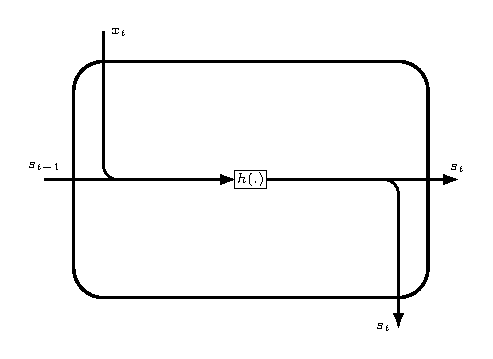
\includegraphics[width=0.48\textwidth]{figures/RNN_cell.pdf}
       \label{fig:rnn_cell}
    }%
  \hfill
  \subfigure[LSTM Cell]{
       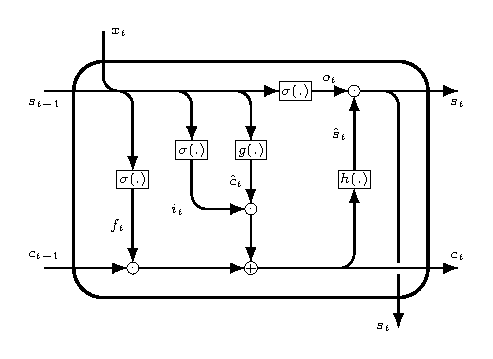
\includegraphics[width=0.48\textwidth]{figures/LSTM_cell.pdf}
       \label{fig:lstm_cell}
  }
    \caption{Cell structures of the RNN and LSTM, respectively}
    \label{fig:cells}
\end{figure}

The forward propagation of the RNN assumes that there is a non-linear activation function at the hidden units. Hidden state of the network is the result of this activation function. 
Outputs are the linear transformations of the hidden states. 
Graphically recurrent neural networks can be shown as Figure~\ref{fig:rnn} with the cell in Figure~\ref{fig:rnn_cell}.
Forward propagation begins with the $s_0$. Then for each time step following update equations will be applied:

\begin{eqnarray}
     s^{\prime}_{t} &=& \mathcal{W}_{ss}s_{t-1} + \mathcal{W}_{sx}x_t + b_s\\ 
     s_{t} &=& h \left(s^{\prime}_{t}\right) \\ 
     \hat{y}_{t} &=& \mathcal{W}_{ys}s_t + c_y
\end{eqnarray}

\begin{figure}
    \centering
    \subfigure{
       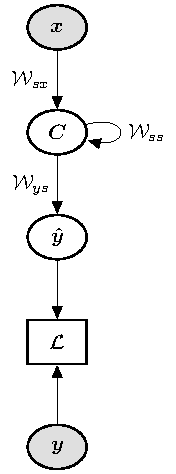
\includegraphics[width=0.231\textwidth]{figures/rnn_folded.pdf}
       \label{fig:rnn_folded}
    }%
  \hfill
  \subfigure{
       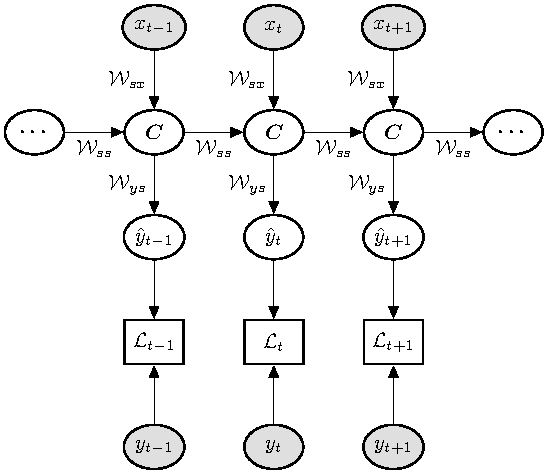
\includegraphics[width=0.7205\textwidth]{figures/rnn_unfolded.pdf}
       \label{fig:rnn_unfolded}
  }
    \caption{Folded and unfolded representation of the computational graphs, respectively}
    \label{fig:rnn}
\end{figure}

By the help of the chain structure and recurrence, these networks can learn sequences and patterns.
However, there are some disadvantages to RNNs. 
Since the gradients are transferred over time and pass through the activation function at each time step, the gradients tend to be decreasing exponentially and disappears after a few time steps. Therefore networks tend to forget the previous inputs after a few time steps and accordingly cannot handle the long-term dependencies.
This problem is usually called as the vanishing gradient \cite{hochreiter1998vanishing}.

\subsection{Long Short-Term Memory}

Learning long-term dependencies in dynamical systems is one of the main challenges in deep learning researches.
Long Short-Term Memory (LSTM) structure is designed for capturing long-term dependencies. 
They remember information for an extended period by default.
Therefore LSTMs have emerged as effective and scalable models for several learning problems related to sequential data \cite{hochreiter1997long}. They are a special kind of RNN that are good at learning long-term dependencies. 
Similar to all kind of RNNs, LSTMs have the form of a chain of repeating modules of neural networks \cite{olah2015understanding}. 

LSTM is a kind of gated RNN. The idea behind the gated RNNs is creating paths through time that have derivatives that neither vanish nor explode \cite{goodfellow2016deep}. Gated RNNs accomplish this idea by the gates that change connection weights at each time step. The central idea behind the LSTM architecture is a memory cell which can maintain its state over time, and non-linear gating units which regulate the information flow into and out of the cell \cite{greff2017lstm}.
The idea of introducing internal recurrence, in addition to the outer recurrence of the RNN, is to produce paths where the gradient can flow for long time-steps.
In standard RNN, repeating structure (cell) has a simple structure, an activation function. On the other hand, LSTM cell has four layers which interact with each other.
The combination of the Figure~\ref{fig:rnn} and Figure~\ref{fig:lstm_cell} could form graphical representation of the LSTMs.
Forward propagation and interactions in the single LSTM cell are derived step by step as following:

\begin{enumerate}
    \item It should be decided which information should be thrown away from the previous cell state. Decision is made by `forget gate' $f_t$. 
    It is derived as follows:
    \begin{eqnarray}
        f_t &=& \sigma\left(\mathcal{W}^{f}_{ss} s_{t-1} + \mathcal{W}_{sx}^{f} x_t + b^f \right)
    \end{eqnarray}
    \item It should be decided which new information coming from input $x_t$ will be stored in new cell state. In order to do this, first a proposal $\hat{c}_t$ should be made for the new cell state and then it should be decided how much of this proposal will be accepted. The decision maker for this process is the `input gate' $i_t$. These are derived as follows:
    \begin{eqnarray}
        \hat{c}_t &=& g\left(\mathcal{W}^{\hat{c}}_{ss} s_{t-1} + \mathcal{W}_{sx}^{\hat{c}} x_t + b^{\hat{c}} \right) \\
        i_t &=& \sigma\left(\mathcal{W}^{i}_{ss} s_{t-1} + \mathcal{W}_{sx}^{i} x_t + b^i \right)
    \end{eqnarray}
    \item The new step is the determination of the new cell state. For this purpose, the outputs obtained in the previous steps should be used. Derivation of the updated cell state is as follows:
    \begin{eqnarray}
        c_t &=& f_t \odot c_{t-1} + i_t \odot \hat{c}_t
    \end{eqnarray}
    \item The new hidden state $s_t$ is calculated after the calculation of the new cell status $c_t$. But this transformation is done in 3 steps. First, the cell state $c_t$ is passed through the activation function $h(.)$ as in RNN and unfiltered hidden state $\hat{s}_t$ is obtained. Then the obtained result is filtered by the `output gate' $o_t$ and the hidden state $s_t$ is obtained . The derivations as follows:
    \begin{eqnarray}
        \hat{s}_t &=& h\left(c_{t}\right) \\
        o_t &=& \sigma\left(\mathcal{W}^{o}_{ss} s_{t-1} + \mathcal{W}_{sx}^{o} x_t + b^o \right) \\
        s_t &=& o_t \odot \hat{s}_t
    \end{eqnarray}
    \item The predictions $\hat{y}_{t}$ of the network are obtained as follows. It is the linear transformation of the hidden state $s_t$ at time $t$, with the output weights of the network $\mathcal{W}_{ys}$, as in RNN.
    \begin{eqnarray}
        \hat{y}_{t} &=& \mathcal{W}_{ys}s_t + c_y
    \end{eqnarray}
\end{enumerate}

LSTMs are the improved version of the RNNs. It has a better capacity of holding past information to current state and known as state of the art sequence model \cite{greff2017lstm}.

\subsection{Learning in RNN and LSTM}

After forward propagation, the loss $\mathcal{L}$ between $y_t$ and $\hat{y}_t$ and gradients will be calculated. Computation of the gradients through an RNN and an LSTM is a straightforward problem\cite{goodfellow2016deep}. A particular version of the backpropagation algorithm, which is known as {\it Backpropagation Through Time} (BPTT), should be applied \cite{werbos1990backpropagation}. 
BPTT operates on an unfolded computational graph of RNN in time. The unfolded network contains $t$ inputs and outputs, but the network shares the same parameters over all networks. Then the backpropagation algorithm is used to find the gradient of the loss function concerning all the network parameters.